% Options for packages loaded elsewhere
\PassOptionsToPackage{unicode}{hyperref}
\PassOptionsToPackage{hyphens}{url}
%
\documentclass[
]{article}
\usepackage{amsmath,amssymb}
\usepackage{lmodern}
\usepackage{iftex}
\ifPDFTeX
  \usepackage[T1]{fontenc}
  \usepackage[utf8]{inputenc}
  \usepackage{textcomp} % provide euro and other symbols
\else % if luatex or xetex
  \usepackage{unicode-math}
  \defaultfontfeatures{Scale=MatchLowercase}
  \defaultfontfeatures[\rmfamily]{Ligatures=TeX,Scale=1}
\fi
% Use upquote if available, for straight quotes in verbatim environments
\IfFileExists{upquote.sty}{\usepackage{upquote}}{}
\IfFileExists{microtype.sty}{% use microtype if available
  \usepackage[]{microtype}
  \UseMicrotypeSet[protrusion]{basicmath} % disable protrusion for tt fonts
}{}
\makeatletter
\@ifundefined{KOMAClassName}{% if non-KOMA class
  \IfFileExists{parskip.sty}{%
    \usepackage{parskip}
  }{% else
    \setlength{\parindent}{0pt}
    \setlength{\parskip}{6pt plus 2pt minus 1pt}}
}{% if KOMA class
  \KOMAoptions{parskip=half}}
\makeatother
\usepackage{xcolor}
\usepackage[margin=1in]{geometry}
\usepackage{color}
\usepackage{fancyvrb}
\newcommand{\VerbBar}{|}
\newcommand{\VERB}{\Verb[commandchars=\\\{\}]}
\DefineVerbatimEnvironment{Highlighting}{Verbatim}{commandchars=\\\{\}}
% Add ',fontsize=\small' for more characters per line
\usepackage{framed}
\definecolor{shadecolor}{RGB}{248,248,248}
\newenvironment{Shaded}{\begin{snugshade}}{\end{snugshade}}
\newcommand{\AlertTok}[1]{\textcolor[rgb]{0.94,0.16,0.16}{#1}}
\newcommand{\AnnotationTok}[1]{\textcolor[rgb]{0.56,0.35,0.01}{\textbf{\textit{#1}}}}
\newcommand{\AttributeTok}[1]{\textcolor[rgb]{0.77,0.63,0.00}{#1}}
\newcommand{\BaseNTok}[1]{\textcolor[rgb]{0.00,0.00,0.81}{#1}}
\newcommand{\BuiltInTok}[1]{#1}
\newcommand{\CharTok}[1]{\textcolor[rgb]{0.31,0.60,0.02}{#1}}
\newcommand{\CommentTok}[1]{\textcolor[rgb]{0.56,0.35,0.01}{\textit{#1}}}
\newcommand{\CommentVarTok}[1]{\textcolor[rgb]{0.56,0.35,0.01}{\textbf{\textit{#1}}}}
\newcommand{\ConstantTok}[1]{\textcolor[rgb]{0.00,0.00,0.00}{#1}}
\newcommand{\ControlFlowTok}[1]{\textcolor[rgb]{0.13,0.29,0.53}{\textbf{#1}}}
\newcommand{\DataTypeTok}[1]{\textcolor[rgb]{0.13,0.29,0.53}{#1}}
\newcommand{\DecValTok}[1]{\textcolor[rgb]{0.00,0.00,0.81}{#1}}
\newcommand{\DocumentationTok}[1]{\textcolor[rgb]{0.56,0.35,0.01}{\textbf{\textit{#1}}}}
\newcommand{\ErrorTok}[1]{\textcolor[rgb]{0.64,0.00,0.00}{\textbf{#1}}}
\newcommand{\ExtensionTok}[1]{#1}
\newcommand{\FloatTok}[1]{\textcolor[rgb]{0.00,0.00,0.81}{#1}}
\newcommand{\FunctionTok}[1]{\textcolor[rgb]{0.00,0.00,0.00}{#1}}
\newcommand{\ImportTok}[1]{#1}
\newcommand{\InformationTok}[1]{\textcolor[rgb]{0.56,0.35,0.01}{\textbf{\textit{#1}}}}
\newcommand{\KeywordTok}[1]{\textcolor[rgb]{0.13,0.29,0.53}{\textbf{#1}}}
\newcommand{\NormalTok}[1]{#1}
\newcommand{\OperatorTok}[1]{\textcolor[rgb]{0.81,0.36,0.00}{\textbf{#1}}}
\newcommand{\OtherTok}[1]{\textcolor[rgb]{0.56,0.35,0.01}{#1}}
\newcommand{\PreprocessorTok}[1]{\textcolor[rgb]{0.56,0.35,0.01}{\textit{#1}}}
\newcommand{\RegionMarkerTok}[1]{#1}
\newcommand{\SpecialCharTok}[1]{\textcolor[rgb]{0.00,0.00,0.00}{#1}}
\newcommand{\SpecialStringTok}[1]{\textcolor[rgb]{0.31,0.60,0.02}{#1}}
\newcommand{\StringTok}[1]{\textcolor[rgb]{0.31,0.60,0.02}{#1}}
\newcommand{\VariableTok}[1]{\textcolor[rgb]{0.00,0.00,0.00}{#1}}
\newcommand{\VerbatimStringTok}[1]{\textcolor[rgb]{0.31,0.60,0.02}{#1}}
\newcommand{\WarningTok}[1]{\textcolor[rgb]{0.56,0.35,0.01}{\textbf{\textit{#1}}}}
\usepackage{graphicx}
\makeatletter
\def\maxwidth{\ifdim\Gin@nat@width>\linewidth\linewidth\else\Gin@nat@width\fi}
\def\maxheight{\ifdim\Gin@nat@height>\textheight\textheight\else\Gin@nat@height\fi}
\makeatother
% Scale images if necessary, so that they will not overflow the page
% margins by default, and it is still possible to overwrite the defaults
% using explicit options in \includegraphics[width, height, ...]{}
\setkeys{Gin}{width=\maxwidth,height=\maxheight,keepaspectratio}
% Set default figure placement to htbp
\makeatletter
\def\fps@figure{htbp}
\makeatother
\setlength{\emergencystretch}{3em} % prevent overfull lines
\providecommand{\tightlist}{%
  \setlength{\itemsep}{0pt}\setlength{\parskip}{0pt}}
\setcounter{secnumdepth}{-\maxdimen} % remove section numbering
\ifLuaTeX
  \usepackage{selnolig}  % disable illegal ligatures
\fi
\IfFileExists{bookmark.sty}{\usepackage{bookmark}}{\usepackage{hyperref}}
\IfFileExists{xurl.sty}{\usepackage{xurl}}{} % add URL line breaks if available
\urlstyle{same} % disable monospaced font for URLs
\hypersetup{
  pdftitle={Compulsory exercise 1: Group 11},
  pdfauthor={Torbjørn Vatne, Ludvik Braathen and Johan Bjerkem},
  hidelinks,
  pdfcreator={LaTeX via pandoc}}

\title{Compulsory exercise 1: Group 11}
\usepackage{etoolbox}
\makeatletter
\providecommand{\subtitle}[1]{% add subtitle to \maketitle
  \apptocmd{\@title}{\par {\large #1 \par}}{}{}
}
\makeatother
\subtitle{TMA4268 Statistical Learning V2023}
\author{Torbjørn Vatne, Ludvik Braathen and Johan Bjerkem}
\date{16 February, 2023}

\begin{document}
\maketitle

\begin{Shaded}
\begin{Highlighting}[]
\FunctionTok{install.packages}\NormalTok{(}\StringTok{"knitr"}\NormalTok{)     }\CommentTok{\# probably already installed}
\FunctionTok{install.packages}\NormalTok{(}\StringTok{"rmarkdown"}\NormalTok{) }\CommentTok{\# probably already installed}
\FunctionTok{install.packages}\NormalTok{(}\StringTok{"ggplot2"}\NormalTok{)   }\CommentTok{\# plotting with ggplot2}
\FunctionTok{install.packages}\NormalTok{(}\StringTok{"dplyr"}\NormalTok{)     }\CommentTok{\# for data cleaning and preparation}
\FunctionTok{install.packages}\NormalTok{(}\StringTok{"tidyr"}\NormalTok{)     }\CommentTok{\# also data preparation}
\FunctionTok{install.packages}\NormalTok{(}\StringTok{"carData"}\NormalTok{)   }\CommentTok{\# dataset}
\FunctionTok{install.packages}\NormalTok{(}\StringTok{"class"}\NormalTok{)     }\CommentTok{\# for KNN}
\FunctionTok{install.packages}\NormalTok{(}\StringTok{"pROC"}\NormalTok{)      }\CommentTok{\# calculate roc}
\FunctionTok{install.packages}\NormalTok{(}\StringTok{"plotROC"}\NormalTok{)   }\CommentTok{\# plot roc}
\FunctionTok{install.packages}\NormalTok{(}\StringTok{"ggmosaic"}\NormalTok{)  }\CommentTok{\# mosaic plot}
\FunctionTok{install.packages}\NormalTok{(}\StringTok{"knitr"}\NormalTok{)}
\FunctionTok{install.packages}\NormalTok{(}\StringTok{"formatR"}\NormalTok{)}
\FunctionTok{library}\NormalTok{(knitr)}
\FunctionTok{install.packages}\NormalTok{(}\StringTok{"tinytex"}\NormalTok{)}
\NormalTok{tinytex}\SpecialCharTok{::}\FunctionTok{install\_tinytex}\NormalTok{()}
\end{Highlighting}
\end{Shaded}

\hypertarget{problem-1-9p}{%
\section{Problem 1 (9P)}\label{problem-1-9p}}

We consider the following regression problem

\[
Y=f(\mathbf {x})+\varepsilon, \text{ where } \text{E}(\varepsilon)=0 \text{ and } \text{Var}(\varepsilon)=\sigma^2.
\]

Assume now that the true function \(f(\mathbf {x})\) is a linear
combination of the observed covariates, that is
\(f(\mathbf{x}) = \mathbf{x}^T\boldsymbol{\beta}=\beta_0 + \beta_1 x_1 + \ldots + \beta_p x_p,\)
where \(\mathbf{x}\) and \(\boldsymbol{\beta}\) are both vectors of
length \(p+1.\)

We know that the OLS estimator in this case is
\(\hat{\boldsymbol{\beta}} = (\mathbf{X}^\top\mathbf{X})^{-1}\mathbf{X}^\top\mathbf{Y}\),
with design matrix \(\mathbf{X}\) and response vector \(\mathbf{Y}\). In
this task we will look at a competing estimator
\(\widetilde{\boldsymbol \beta} =(\mathbf{X}^\top\mathbf{X}+\lambda {\bf I})^{-1}\mathbf{X}^\top{\bf Y}\)
(this is called the ridge regression estimator), where \(\lambda\ge0\)
is a constant tuning parameter that controls the bias-variance
trade-off. Observe that for \(\lambda = 0\) the ridge regression
estimator is equivalent to \(\hat{\boldsymbol{\beta}}.\)

We will first derive mathematical formulas for the bias and variance of
\(\widetilde{\boldsymbol \beta}\) and then we will plot these curves in
R.

\hypertarget{a-1p}{%
\subsection{a) (1P)}\label{a-1p}}

Find the expected value and the variance-covariance matrix of
\(\widetilde{\boldsymbol \beta}.\)

Here we find the expected value:

\[
\displaylines{
    E(\widetilde{\boldsymbol \beta})=E((\mathbf{X}^\top\mathbf{X}+\lambda {\bf I})^{-1}\mathbf{X}^\top{\bf Y})\cr
    E(\widetilde{\boldsymbol \beta})=(\mathbf{X}^\top\mathbf{X}+\lambda {\bf I})^{-1}\mathbf{X}^\top{E(\bf Y})\cr
    E(\widetilde{\boldsymbol \beta})=(\mathbf{X}^\top\mathbf{X}+\lambda {\bf I})^{-1}\mathbf{X}^\top{E(\bf X \boldsymbol \beta + \varepsilon})\cr
    E(\widetilde{\boldsymbol \beta})=(\mathbf{X}^\top\mathbf{X}+\lambda {\bf I})^{-1}\mathbf{X}^\top{(\bf X \boldsymbol \beta + 0})\cr
    E(\widetilde{\boldsymbol \beta})=(\mathbf{X}^\top\mathbf{X}+\lambda {\bf I})^{-1}\mathbf{X}^\top{\bf X \boldsymbol \beta}\cr
}
\] Here we find the variance-covarince matrix:

\begin{align}
Cov(\widetilde{\boldsymbol \beta})&=Cov((X^T X + \lambda I)^{-1}X^T Y)\\
&=(X^T X + \lambda I)^{-1}X^T Cov(Y)((X^TX + \lambda I)^{-1}X^T)^T \\
&=(X^TX + \lambda I)^{-1}X^T \sigma^2  I ((X^TX + \lambda I)^{-1}X^T)^T
\end{align}

\hypertarget{b-2p}{%
\subsection{b) (2P)}\label{b-2p}}

Let
\(\widetilde{f}(\mathbf{x}_0)=\mathbf{x}_0^T \widetilde{\boldsymbol{\beta}}\)
be the prediction at a new covariate vector \(\mathbf{x}_0.\) Using a),
find the expected value and variance for
\(\widetilde{f}(\mathbf{x}_0)=\mathbf{x}_0^T \widetilde{\boldsymbol{\beta}}.\)

First we find the expecrted value:

\[
\displaylines{
    E(\mathbf{x}_0^T \widetilde{\boldsymbol{\beta}})=\mathbf{x}_0^T E(\widetilde{\boldsymbol{\beta}})\cr
    E(\mathbf{x}_0^T \widetilde{\boldsymbol{\beta}})=\mathbf{x}_0^T (\mathbf{X}^\top\mathbf{X}+\lambda {\bf I})^{-1}\mathbf{X}^\top{\bf X \boldsymbol \beta}\cr
}
\] Then we find the variance: (Here we need to remember the rule for
variance where we need to multiply the same term transposed at the back
of the variance term.)

\[
\displaylines{
    Var(\mathbf{x}_0^T \widetilde{\boldsymbol{\beta}})=\mathbf{x}_0^T Var(\widetilde{\boldsymbol{\beta}}) \mathbf{x}_0\cr
    Var(\mathbf{x}_0^T \widetilde{\boldsymbol{\beta}})=\mathbf{x}_0^T Var(\widetilde{\boldsymbol{\beta}}) \mathbf{x}_0\cr
     Var(\mathbf{x}_0^T \widetilde{\boldsymbol{\beta}})=\mathbf{x}_0^T (\mathbf{X}^\top\mathbf{X}+\lambda {\bf I})^{-1}\mathbf{X}^\top{\sigma^2}((\mathbf{X}^\top\mathbf{X}+\lambda {\bf I})^{-1}\mathbf{X}^\top)^\top \mathbf{x}_0
}
\]

\hypertarget{c-1p}{%
\subsection{c) (1P)}\label{c-1p}}

Explain with words how we can interpret the three terms: bias, variance
and irreducible error.

Bias is the error that comes by oversimplifying the model. This means
underfitting the model, meaning high bias will over simplify the
relationships in the data. Variance, on the other hand, is the error
that comes by creating a too complex mode. This means overfitting the
model, where the model tries to hard to fit the function to the noise of
the data. There is a famous plot of the relationship between bias and
variance. When we train a model we start with a high bias that decays as
we train the model. The variance starts low and increases as we train
the model. We want to hit the sweet spot where bias and variance
intercepts, as this is the point with the minimal total error.
Irreducible error is the error that comes with the data. As the name
suggests this error cannot be eliminated by any model, as it is inherit
by the data and is not due to bias or variance.

\hypertarget{d-2p}{%
\subsection{d) (2P)}\label{d-2p}}

Find the expected MSE at \(\mathbf{x}_0,\)
\(E[(y_0 - \widetilde{f}(\mathbf{x}_0))^2]\).

\emph{Hint}: Use that the expected MSE can be decomposed into squared
bias, variance and irreducible error, and then move on from there.

\$\$ \displaylines{
    E[(y_0 - \widetilde{f}(\mathbf{x}_0))^2]=Var(\widetilde{f}(\mathbf{x}_0)) + (Bias(\widetilde{f}(\mathbf{x}_0)))^2 + Var(\varepsilon)\cr\cr
    
    Var(\widetilde{f}(\mathbf{x}_0)) = \mathbf{x}_0^T (\mathbf{X}^\top\mathbf{X}+\lambda {\bf I})^{-1}\mathbf{X}^\top{\sigma^2}((\mathbf{X}^\top\mathbf{X}+\lambda {\bf I})^{-1}\mathbf{X}^\top)^\top \mathbf{x}_0\cr\cr
    
    (Bias(\widetilde{f}(\mathbf{x}_0)))^2 = (E(\mathbf{y}_0 - \widetilde{f}(\mathbf{x}_0)))^2\cr\
    (Bias(\widetilde{f}(\mathbf{x}_0)))^2 = (E(\mathbf{y}_0) - E(\widetilde{f}(\mathbf{x}_0)))^2\cr
        (Bias(\widetilde{f}(\mathbf{x}_0)))^2 = (\mathbf{y}_0 - \mathbf{x}_0^T (\mathbf{X}^\top\mathbf{X}+\lambda {\bf I})^{-1}\mathbf{X}^\top{\bf X \boldsymbol \beta})^2\cr\cr

    Var(\varepsilon) = {\sigma^2}\cr\cr
    E[(y_0 - \widetilde{f}(\mathbf{x}_0))^2]=\mathbf{x}_0^T (\mathbf{X}^\top\mathbf{X}+\lambda {\bf I})^{-1}\mathbf{X}^\top{\sigma^2}((\mathbf{X}^\top\mathbf{X}+\lambda {\bf I})^{-1}\mathbf{X}^\top)^\top \mathbf{x}_0 + (Bias(\widetilde{f}(\mathbf{x}_0)))^2 + {\sigma^2}\cr
} E{[}(y\_0 - \widetilde{f}(\mathbf{x}\_0))\^{}2{]}=\mathbf{x}\_0\^{}T
(\mathbf{X}\textsuperscript{\top\mathbf{X}+\lambda {\bf I})}\{-1\}\mathbf{X}\textsuperscript{\top{\sigma^2}((\mathbf{X}}\top\mathbf{X}+\lambda {\bf I})\textsuperscript{\{-1\}\mathbf{X}}\top)\^{}\top \mathbf{x}\_0
+ (Bias(\widetilde{f}(\mathbf{x}\_0)))\^{}2 + \{\sigma\^{}2\}\cr \} \$\$

\hypertarget{plotting-the-bias-variance-trade-off}{%
\subsubsection{Plotting the bias-variance
trade-off}\label{plotting-the-bias-variance-trade-off}}

The estimator \(\widetilde{\boldsymbol\beta}\) is a function of the
tuning parameter \(\lambda\), which controls the bias-variance
trade-off. Using the decomposition derived in c) we will plot the three
elements (bias, variance and irreducible error) using the values in the
code chunk below. \texttt{values} is a list with the design matrix
\texttt{X}, the vector \(\mathbf{x}_0\) as \texttt{x0}, the parameters
vector \texttt{beta} and the irreducible error \texttt{sigma}.

\begin{Shaded}
\begin{Highlighting}[]
\NormalTok{id }\OtherTok{\textless{}{-}} \StringTok{"1X\_8OKcoYbng1XvYFDirxjEWr7LtpNr1m"} \CommentTok{\# google file ID}
\NormalTok{values }\OtherTok{\textless{}{-}} \FunctionTok{dget}\NormalTok{(}\FunctionTok{sprintf}\NormalTok{(}\StringTok{"https://docs.google.com/uc?id=\%s\&export=download"}\NormalTok{, id))}
\NormalTok{X }\OtherTok{\textless{}{-}}\NormalTok{ values}\SpecialCharTok{$}\NormalTok{X}
\FunctionTok{dim}\NormalTok{(X)}
\end{Highlighting}
\end{Shaded}

\begin{verbatim}
## [1] 100  81
\end{verbatim}

\begin{Shaded}
\begin{Highlighting}[]
\NormalTok{x0 }\OtherTok{\textless{}{-}}\NormalTok{ values}\SpecialCharTok{$}\NormalTok{x0}
\FunctionTok{dim}\NormalTok{(x0)}
\end{Highlighting}
\end{Shaded}

\begin{verbatim}
## [1] 81  1
\end{verbatim}

\begin{Shaded}
\begin{Highlighting}[]
\NormalTok{beta }\OtherTok{\textless{}{-}}\NormalTok{ values}\SpecialCharTok{$}\NormalTok{beta}
\FunctionTok{dim}\NormalTok{(beta)}
\end{Highlighting}
\end{Shaded}

\begin{verbatim}
## [1] 81  1
\end{verbatim}

\begin{Shaded}
\begin{Highlighting}[]
\NormalTok{sigma }\OtherTok{\textless{}{-}}\NormalTok{ values}\SpecialCharTok{$}\NormalTok{sigma}
\NormalTok{sigma}
\end{Highlighting}
\end{Shaded}

\begin{verbatim}
## [1] 0.5
\end{verbatim}

\hypertarget{e-1p}{%
\subsection{e) (1P)}\label{e-1p}}

First we will create the squared bias function (\texttt{bias}) which
takes as inputs the parameter \texttt{lambda}, \texttt{X}, \texttt{x0},
\texttt{beta} and returns the squared bias. You have only to fill the
\texttt{value\ \textless{}-\ ...} and run the chunk of code to plot the
squared bias, where value is the squared bias as derived in d).

\begin{Shaded}
\begin{Highlighting}[]
\FunctionTok{library}\NormalTok{(ggplot2)}
\NormalTok{bias }\OtherTok{\textless{}{-}} \ControlFlowTok{function}\NormalTok{(lambda, X, x0, beta) \{}
\NormalTok{  p }\OtherTok{\textless{}{-}} \FunctionTok{ncol}\NormalTok{(X)}
\NormalTok{  inv }\OtherTok{\textless{}{-}} \FunctionTok{solve}\NormalTok{(}\FunctionTok{t}\NormalTok{(X) }\SpecialCharTok{\%*\%}\NormalTok{ X }\SpecialCharTok{+}\NormalTok{ lambda }\SpecialCharTok{*} \FunctionTok{diag}\NormalTok{(p))}
\NormalTok{  value }\OtherTok{\textless{}{-}}\NormalTok{ (}\FunctionTok{t}\NormalTok{(x0)}\SpecialCharTok{\%*\%}\NormalTok{(}\FunctionTok{t}\NormalTok{(X)}\SpecialCharTok{\%*\%}\NormalTok{X}\SpecialCharTok{{-}}\NormalTok{lambda}\SpecialCharTok{*}\FunctionTok{diag}\NormalTok{(p))}\SpecialCharTok{\^{}{-}}\DecValTok{1}\SpecialCharTok{\%*\%}\FunctionTok{t}\NormalTok{(X)}\SpecialCharTok{\%*\%}\NormalTok{X}\SpecialCharTok{\%*\%}\NormalTok{beta)}\SpecialCharTok{\^{}}\DecValTok{2}
  \FunctionTok{return}\NormalTok{(value)}
\NormalTok{\}}
\NormalTok{lambdas }\OtherTok{\textless{}{-}} \FunctionTok{seq}\NormalTok{(}\DecValTok{0}\NormalTok{, }\DecValTok{2}\NormalTok{, }\AttributeTok{length.out =} \DecValTok{500}\NormalTok{)}
\NormalTok{BIAS }\OtherTok{\textless{}{-}} \FunctionTok{rep}\NormalTok{(}\ConstantTok{NA}\NormalTok{, }\FunctionTok{length}\NormalTok{(lambdas))}
\ControlFlowTok{for}\NormalTok{ (i }\ControlFlowTok{in} \FunctionTok{seq\_along}\NormalTok{(lambdas)) BIAS[i] }\OtherTok{\textless{}{-}} \FunctionTok{bias}\NormalTok{(lambdas[i], X, x0, beta)}
\NormalTok{dfBias }\OtherTok{\textless{}{-}} \FunctionTok{data.frame}\NormalTok{(}\AttributeTok{lambdas =}\NormalTok{ lambdas, }\AttributeTok{bias =}\NormalTok{ BIAS)}
\FunctionTok{ggplot}\NormalTok{(dfBias, }\FunctionTok{aes}\NormalTok{(}\AttributeTok{x =}\NormalTok{ lambdas, }\AttributeTok{y =}\NormalTok{ bias)) }\SpecialCharTok{+}
  \FunctionTok{geom\_line}\NormalTok{(}\AttributeTok{color =} \StringTok{"hotpink"}\NormalTok{) }\SpecialCharTok{+}
  \FunctionTok{xlab}\NormalTok{(}\FunctionTok{expression}\NormalTok{(lambda)) }\SpecialCharTok{+}
  \FunctionTok{ylab}\NormalTok{(}\FunctionTok{expression}\NormalTok{(bias}\SpecialCharTok{\^{}}\DecValTok{2}\NormalTok{))}
\end{Highlighting}
\end{Shaded}

\hypertarget{f-1p}{%
\subsection{f) (1P)}\label{f-1p}}

Now we will create the variance function which takes the same inputs as
the squared bias. As in e) you have to fill only the
\texttt{value\ \textless{}-\ ...} and run the code to plot the variance.

\begin{Shaded}
\begin{Highlighting}[]
\NormalTok{variance }\OtherTok{\textless{}{-}} \ControlFlowTok{function}\NormalTok{(lambda, X, x0, sigma) \{}
\NormalTok{  p }\OtherTok{\textless{}{-}} \FunctionTok{ncol}\NormalTok{(X)}
\NormalTok{  inv }\OtherTok{\textless{}{-}} \FunctionTok{solve}\NormalTok{(}\FunctionTok{t}\NormalTok{(X) }\SpecialCharTok{\%*\%}\NormalTok{ X }\SpecialCharTok{+}\NormalTok{ lambda }\SpecialCharTok{*} \FunctionTok{diag}\NormalTok{(p))}
  \FunctionTok{print}\NormalTok{(inv)}
\NormalTok{  value }\OtherTok{\textless{}{-}}\NormalTok{ ...}
  \FunctionTok{return}\NormalTok{(value)}
\NormalTok{\}}
\NormalTok{lambdas }\OtherTok{\textless{}{-}} \FunctionTok{seq}\NormalTok{(}\DecValTok{0}\NormalTok{, }\DecValTok{2}\NormalTok{, }\AttributeTok{length.out =} \DecValTok{500}\NormalTok{)}
\NormalTok{VAR }\OtherTok{\textless{}{-}} \FunctionTok{rep}\NormalTok{(}\ConstantTok{NA}\NormalTok{, }\FunctionTok{length}\NormalTok{(lambdas))}
\ControlFlowTok{for}\NormalTok{ (i }\ControlFlowTok{in} \FunctionTok{seq\_along}\NormalTok{(lambdas)) VAR[i] }\OtherTok{\textless{}{-}} \FunctionTok{variance}\NormalTok{(lambdas[i], X, x0, sigma)}
\NormalTok{dfVar }\OtherTok{\textless{}{-}} \FunctionTok{data.frame}\NormalTok{(}\AttributeTok{lambdas =}\NormalTok{ lambdas, }\AttributeTok{var =}\NormalTok{ VAR)}
\FunctionTok{ggplot}\NormalTok{(dfVar, }\FunctionTok{aes}\NormalTok{(}\AttributeTok{x =}\NormalTok{ lambdas, }\AttributeTok{y =}\NormalTok{ var)) }\SpecialCharTok{+}
  \FunctionTok{geom\_line}\NormalTok{(}\AttributeTok{color =} \StringTok{"gold"}\NormalTok{) }\SpecialCharTok{+}
  \FunctionTok{xlab}\NormalTok{(}\FunctionTok{expression}\NormalTok{(lambda)) }\SpecialCharTok{+}
  \FunctionTok{ylab}\NormalTok{(}\StringTok{"variance"}\NormalTok{)}
\end{Highlighting}
\end{Shaded}

\hypertarget{g-1p}{%
\subsection{g) (1P)}\label{g-1p}}

Fill in the \texttt{exp\_mse} of the following code to calculate the
expected MSE for the same lambda values that you plugged in above. Then
plot all the components together and find the value of \(\lambda\) which
minimizes the expected MSE.

\begin{Shaded}
\begin{Highlighting}[]
\NormalTok{exp\_mse }\OtherTok{\textless{}{-}}\NormalTok{ ...}
\NormalTok{lambdas[}\FunctionTok{which.min}\NormalTok{(exp\_mse)]}
\end{Highlighting}
\end{Shaded}

\hypertarget{problem-2-15p}{%
\section{Problem 2 (15P)}\label{problem-2-15p}}

Bert-Ernie has his eye on a career in academia, but has not really
decided on a field yet. Like most academics, his greatest concern is his
future salary as a tenured professor. He comes across the
\texttt{Salaries} dataset from the \texttt{carData} \texttt{R} package,
and decides to perform a statistical analysis to try to find out how he
can maximize his future salary as an academic.

To get more information about the covariates in the dataset, you should
run \texttt{?Salaries} after loading the data. It's also a good idea to
do a \emph{descriptive analysis} of the data before fitting any models.
A good starting point can be the \texttt{ggpairs()} function from the
\texttt{GGally} package.

\begin{Shaded}
\begin{Highlighting}[]
\FunctionTok{library}\NormalTok{(carData)}
\NormalTok{GGally}\SpecialCharTok{::}\FunctionTok{ggpairs}\NormalTok{(Salaries)}
\end{Highlighting}
\end{Shaded}

\begin{figure}

{\centering 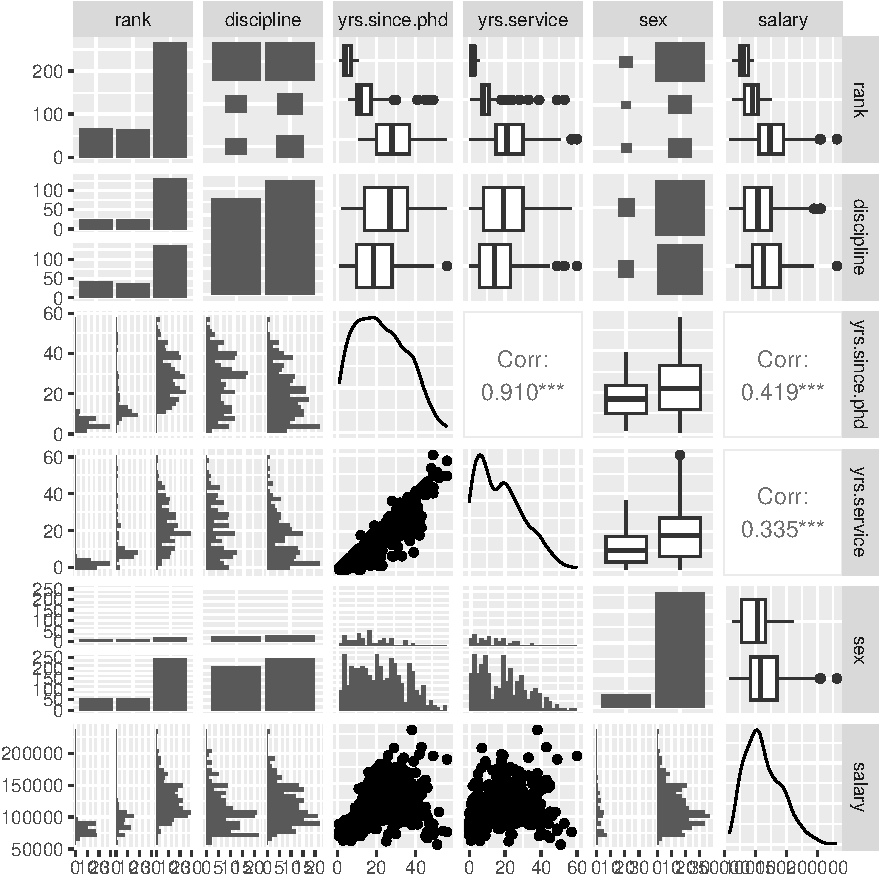
\includegraphics[width=0.7\linewidth]{compulsory_files/figure-latex/desc-1} 

}

\caption{Pairs plot of the academic salary data set.}\label{fig:desc}
\end{figure}

After doing a descriptive analysis, Bert-Ernie makes a multiple linear
regression model with all covariates included, which he calls
\texttt{model1}.

\begin{Shaded}
\begin{Highlighting}[]
\CommentTok{\# Fit full model}
\NormalTok{?Salaries}
\NormalTok{model1 }\OtherTok{\textless{}{-}} \FunctionTok{lm}\NormalTok{(salary }\SpecialCharTok{\textasciitilde{}}\NormalTok{ rank }\SpecialCharTok{+}\NormalTok{ discipline }\SpecialCharTok{+}\NormalTok{ yrs.since.phd }\SpecialCharTok{+}\NormalTok{ yrs.service }\SpecialCharTok{+}\NormalTok{ sex, }\AttributeTok{data =}\NormalTok{ Salaries)}
\FunctionTok{summary}\NormalTok{(model1)}
\end{Highlighting}
\end{Shaded}

\begin{verbatim}
## 
## Call:
## lm(formula = salary ~ rank + discipline + yrs.since.phd + yrs.service + 
##     sex, data = Salaries)
## 
## Residuals:
##    Min     1Q Median     3Q    Max 
## -65248 -13211  -1775  10384  99592 
## 
## Coefficients:
##               Estimate Std. Error t value Pr(>|t|)    
## (Intercept)    65955.2     4588.6  14.374  < 2e-16 ***
## rankAssocProf  12907.6     4145.3   3.114  0.00198 ** 
## rankProf       45066.0     4237.5  10.635  < 2e-16 ***
## disciplineB    14417.6     2342.9   6.154 1.88e-09 ***
## yrs.since.phd    535.1      241.0   2.220  0.02698 *  
## yrs.service     -489.5      211.9  -2.310  0.02143 *  
## sexMale         4783.5     3858.7   1.240  0.21584    
## ---
## Signif. codes:  0 '***' 0.001 '**' 0.01 '*' 0.05 '.' 0.1 ' ' 1
## 
## Residual standard error: 22540 on 390 degrees of freedom
## Multiple R-squared:  0.4547, Adjusted R-squared:  0.4463 
## F-statistic:  54.2 on 6 and 390 DF,  p-value: < 2.2e-16
\end{verbatim}

\begin{Shaded}
\begin{Highlighting}[]
\FunctionTok{plot}\NormalTok{(model1)}
\end{Highlighting}
\end{Shaded}

\begin{center}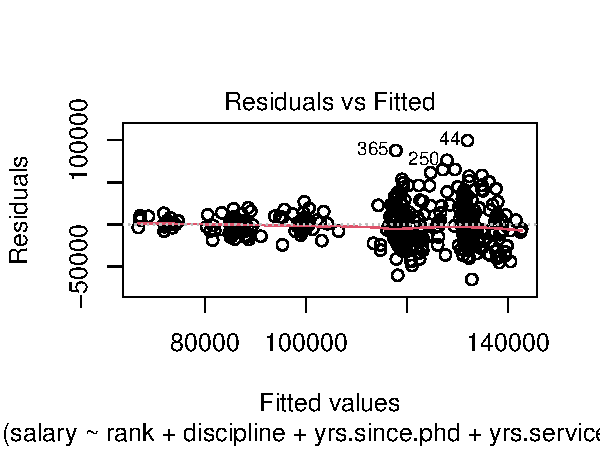
\includegraphics{compulsory_files/figure-latex/load_data-1} \end{center}

\begin{center}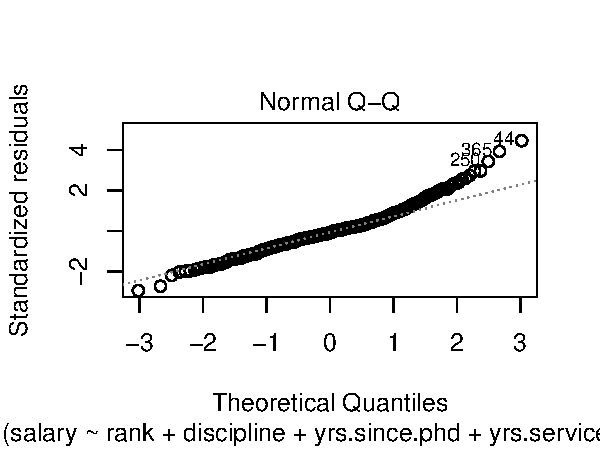
\includegraphics{compulsory_files/figure-latex/load_data-2} \end{center}

\begin{center}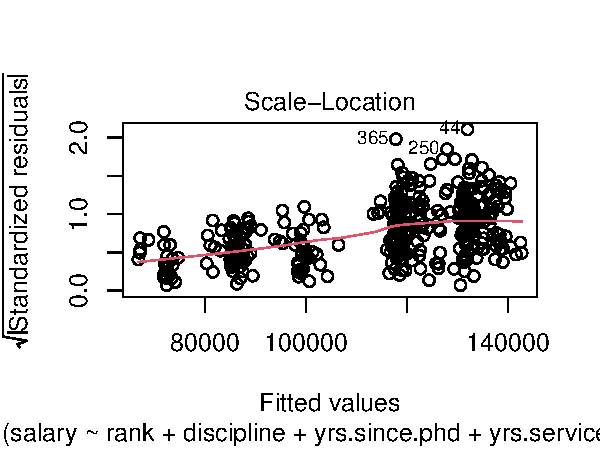
\includegraphics{compulsory_files/figure-latex/load_data-3} \end{center}

\begin{center}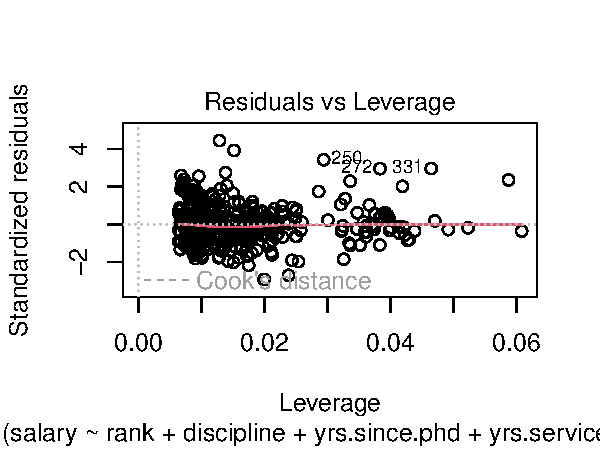
\includegraphics{compulsory_files/figure-latex/load_data-4} \end{center}

\hypertarget{a-categorical-variables-2p}{%
\subsection{a) Categorical variables
(2P)}\label{a-categorical-variables-2p}}

The covariate \texttt{rank} is categorical, with the three possible
values \texttt{AsstProf} (assistant professor), \texttt{AssocProf}
(associate professor) and \texttt{Prof} (full professor).

\begin{enumerate}
\def\labelenumi{\roman{enumi})}
\tightlist
\item
  How does the \texttt{lm()} function encode for this type of covariate,
  and what are the interpretations of the \texttt{rankAssocProf} and
  \texttt{rankProf} estimates, respectively? (1P)
\end{enumerate}

FIKS FORMATERING The \(lm()\) function by default uses the first of the
three levels (of the covariate rank), \texttt{AsstProf}, as a reference
level, and then converts the other levels, \texttt{AssocProf} and
\texttt{Prof}, to a set of `dummy variables'. These dummy variables are
represented as binary variables. Naturally, only one of the levels can
be `active' at once, as a professor can only be either of the three
different types of professors. The estimated coefficient for associate
professor represents the difference in mean salary between associate
professors and assistant professors (reference level), while the
estimated coefficient for a full professor represents the difference in
mean salary between full professors and assistant professors. In other
words, associate professors are expected to earn at average 12907 more
than an assistant professor, and full professors are expected to earn at
average 45066 more than an assistant professor.

The output from \texttt{summary()} tells us the \(p\)-values of
\texttt{rankAssocProf} and \texttt{rankProf}, but not \texttt{rank} as a
whole.

\begin{enumerate}
\def\labelenumi{\roman{enumi})}
\setcounter{enumi}{1}
\tightlist
\item
  Perform an appropriate test to check whether there is evidence that
  \texttt{rank} as a whole has an impact on \texttt{salary}. The output
  from \texttt{summary()} is not enough to do this. (1P)
\end{enumerate}

\begin{Shaded}
\begin{Highlighting}[]
\FunctionTok{library}\NormalTok{(carData)}
\NormalTok{r.salary.rank }\OtherTok{\textless{}{-}} \FunctionTok{lm}\NormalTok{(salary }\SpecialCharTok{\textasciitilde{}}\NormalTok{ yrs.service }\SpecialCharTok{+}\NormalTok{ yrs.since.phd }\SpecialCharTok{+}\NormalTok{ rank , }\AttributeTok{data =}\NormalTok{ Salaries)}
\NormalTok{r.salary.no.rank }\OtherTok{\textless{}{-}} \FunctionTok{lm}\NormalTok{(salary }\SpecialCharTok{\textasciitilde{}}\NormalTok{ yrs.service }\SpecialCharTok{+}\NormalTok{ yrs.since.phd, }\AttributeTok{data =}\NormalTok{ Salaries)}
\FunctionTok{anova}\NormalTok{(r.salary.rank, r.salary.no.rank)}
\end{Highlighting}
\end{Shaded}

\begin{verbatim}
## Analysis of Variance Table
## 
## Model 1: salary ~ yrs.service + yrs.since.phd + rank
## Model 2: salary ~ yrs.service + yrs.since.phd
##   Res.Df        RSS Df   Sum of Sq      F    Pr(>F)    
## 1    392 2.1839e+11                                    
## 2    394 2.9487e+11 -2 -7.6488e+10 68.648 < 2.2e-16 ***
## ---
## Signif. codes:  0 '***' 0.001 '**' 0.01 '*' 0.05 '.' 0.1 ' ' 1
\end{verbatim}

Here we've done a comparison of two models, Model 1 and Model 2. In
Model 1 we've included the variables: \texttt{yrs.service},
\texttt{yrs.since.PhD}, and \texttt{rank}. In Model 2 we also include
\texttt{yrs.service} and \texttt{yrs.since.PhD}, but excluded the
\texttt{rank}-variable. Running \(anova()\) on these two models, gives
us an \(F\)-value of 68.648 and a \(p\)-value of 2.2e-16. Determining
which values of an F-test that are considered `good' is not easy. In
this case, with a relatively high \(F\)-value, together with a
\(p\)-value which is practically 0, we consider that there is enough
evidence that \texttt{rank} as a whole does have an impact on
\texttt{salary}.

\hypertarget{b-conflicting-model-results-2p}{%
\subsection{b) Conflicting model results?
(2P)}\label{b-conflicting-model-results-2p}}

Having heard of the gender wage-gap, Bert-Ernie is surprised to see that
\texttt{model1} finds no evidence that \texttt{sex} has an effect on
\texttt{salary}. To make sure nothing has gone wrong, he fits a new
model with \texttt{sex} as the only covariate (along with an intercept).

\begin{Shaded}
\begin{Highlighting}[]
\FunctionTok{library}\NormalTok{(ggplot2)}
\NormalTok{sex\_model }\OtherTok{\textless{}{-}} \FunctionTok{lm}\NormalTok{(salary }\SpecialCharTok{\textasciitilde{}}\NormalTok{ sex, }\AttributeTok{data =}\NormalTok{ Salaries)}
\FunctionTok{summary}\NormalTok{(sex\_model)}
\end{Highlighting}
\end{Shaded}

\begin{verbatim}
## 
## Call:
## lm(formula = salary ~ sex, data = Salaries)
## 
## Residuals:
##    Min     1Q Median     3Q    Max 
## -57290 -23502  -6828  19710 116455 
## 
## Coefficients:
##             Estimate Std. Error t value Pr(>|t|)    
## (Intercept)   101002       4809  21.001  < 2e-16 ***
## sexMale        14088       5065   2.782  0.00567 ** 
## ---
## Signif. codes:  0 '***' 0.001 '**' 0.01 '*' 0.05 '.' 0.1 ' ' 1
## 
## Residual standard error: 30030 on 395 degrees of freedom
## Multiple R-squared:  0.01921,    Adjusted R-squared:  0.01673 
## F-statistic: 7.738 on 1 and 395 DF,  p-value: 0.005667
\end{verbatim}

\begin{Shaded}
\begin{Highlighting}[]
\FunctionTok{ggplot}\NormalTok{(Salaries, }\FunctionTok{aes}\NormalTok{(}\AttributeTok{x =}\NormalTok{ sex, }\AttributeTok{y =}\NormalTok{ salary, }\AttributeTok{color =}\NormalTok{ rank)) }\SpecialCharTok{+}
  \FunctionTok{geom\_jitter}\NormalTok{() }\SpecialCharTok{+}
  \FunctionTok{labs}\NormalTok{(}\AttributeTok{x =} \StringTok{"Sex"}\NormalTok{, }\AttributeTok{y =} \StringTok{"Salary"}\NormalTok{, }\AttributeTok{color =} \StringTok{"Rank"}\NormalTok{) }\SpecialCharTok{+}
  \FunctionTok{scale\_x\_discrete}\NormalTok{(}\AttributeTok{labels =} \FunctionTok{c}\NormalTok{(}\StringTok{"Female"}\NormalTok{, }\StringTok{"Male"}\NormalTok{))}
\end{Highlighting}
\end{Shaded}

\begin{center}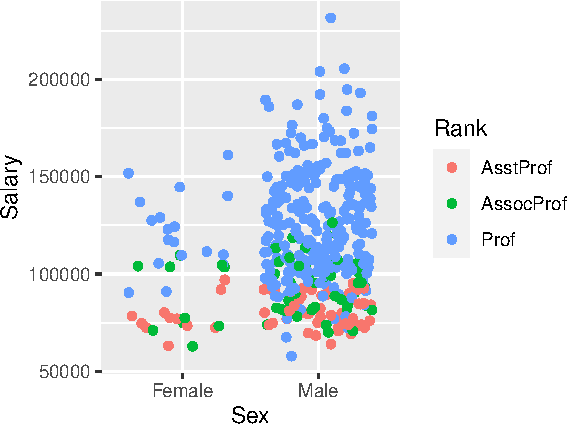
\includegraphics{compulsory_files/figure-latex/sex_model_with_rank-1} \end{center}

\begin{Shaded}
\begin{Highlighting}[]
\NormalTok{sex\_model }\OtherTok{\textless{}{-}} \FunctionTok{lm}\NormalTok{(salary }\SpecialCharTok{\textasciitilde{}}\NormalTok{ sex, }\AttributeTok{data =}\NormalTok{ Salaries)}
\FunctionTok{boxplot}\NormalTok{(salary}\SpecialCharTok{\textasciitilde{}}\NormalTok{sex, }\AttributeTok{data=}\NormalTok{Salaries)}
\end{Highlighting}
\end{Shaded}

\begin{center}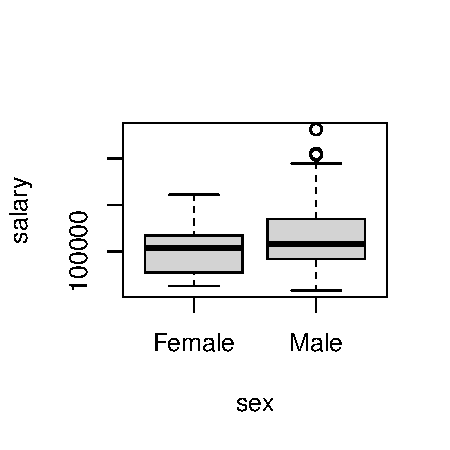
\includegraphics{compulsory_files/figure-latex/sex_model_without_rank-1} \end{center}

The new model finds strong evidence that \texttt{sex} has an effect on
\texttt{salary}. How would you explain the fact that \texttt{sex\_model}
finds evidence of \texttt{sex} impacting \texttt{salary}, but the full
model \texttt{model1} does not? Make one or two figures to demonstrate
your explanation, with proper figure captions explaining the figure(s).
(2P)

SVAR TIL B): A possibility is that the relationship between sex and
salary is confounded with other variables in the full model. This might
happen when another variable is associated with both the predictor (sex)
and the outcome (salary), causing the apparent relationship between the
predictor and outcome to `lie'. To try and demonstrate this, we first
created a a scatter-plot which shows the salary of men and women, with
different colors representing the different levels of rank. We also
created a box-plot of the salary for men and women, but without
consideration of the rank. The box-plot clearly shows that there's a
difference between the salary for men and women. Though when we compare
the box-plot to the scatter-plot, we see\ldots\ldots\ldots.

\textbf{Hint}: The descriptive analysis might be useful to identify what
is going on.

\hypertarget{c-model-assumptions-and-transformation-2p}{%
\subsection{c) Model assumptions and transformation
(2P)}\label{c-model-assumptions-and-transformation-2p}}

Checking the assumptions of \texttt{model1}, Bert-Ernie observes that
the assumptions of the linear regression model are not fulfilled in
\texttt{model1}.

\begin{Shaded}
\begin{Highlighting}[]
\FunctionTok{library}\NormalTok{(ggplot2)}
\FunctionTok{library}\NormalTok{(ggfortify)}
\FunctionTok{autoplot}\NormalTok{(model1, }\AttributeTok{smooth.colour =} \ConstantTok{NA}\NormalTok{)}
\end{Highlighting}
\end{Shaded}

\begin{figure}

{\centering 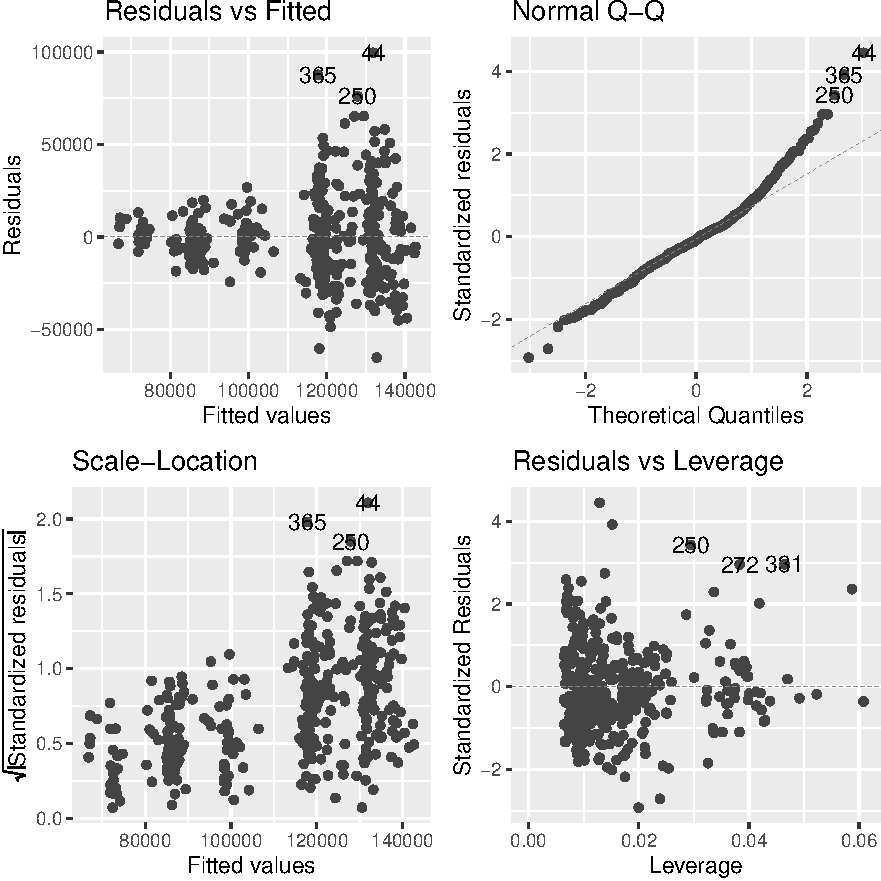
\includegraphics[width=0.6\linewidth]{compulsory_files/figure-latex/fig_model_check-1} 

}

\caption{Diagnostic plots for `model1`.}\label{fig:fig_model_check}
\end{figure}

\begin{enumerate}
\def\labelenumi{\roman{enumi})}
\tightlist
\item
  Based on the figure below, which assumptions are not fulfilled? (1P)
\end{enumerate}

Residuals vs fitted: We can clearly see that the expected value of the
residuals are zero, which fulfills the first assumption. It looks like
the variance of the residuals increase as the salary/fitted values
increase, which does not fulfill the second assumption.

Normal Q-Q: From this plot the residuals seems fairly normal
distributed, at least up until\ldots\ldots\ldots{}

Scale-location: We again see a pattern where the variance of the
residuals increase as the salary/fitted values increase, which can
confirm our earlier conclusion about the second assumption not being
fulfilled.

Residual vs leverage: There is a couple of outliers with high leverage,
Cooks-distance\ldots\ldots{}

\begin{enumerate}
\def\labelenumi{\roman{enumi})}
\setcounter{enumi}{1}
\tightlist
\item
  Bert-Ernie has heard that sometimes such issues may be solved by
  transforming the response or covariates of the model, so he decides to
  try treating the log-transform of \texttt{salary} as the response in a
  new model. Implement the new model, and call it \texttt{model2}. Have
  the model assumptions improved in \texttt{model2} compared to
  \texttt{model1}? (1P)
\end{enumerate}

\begin{Shaded}
\begin{Highlighting}[]
\NormalTok{log\_salary }\OtherTok{\textless{}{-}} \FunctionTok{log}\NormalTok{(Salaries}\SpecialCharTok{$}\NormalTok{salary)}
\CommentTok{\#Får feilmelding under knitting (pga log\_salary elns) dersom jeg skriver det slik:}
\CommentTok{\#model2 \textless{}{-} lm(log\_salary \textasciitilde{} . {-}salary)}
\NormalTok{model2 }\OtherTok{\textless{}{-}} \FunctionTok{lm}\NormalTok{(log\_salary }\SpecialCharTok{\textasciitilde{}}\NormalTok{ rank }\SpecialCharTok{+}\NormalTok{ discipline }\SpecialCharTok{+}\NormalTok{ yrs.since.phd }\SpecialCharTok{+}\NormalTok{ yrs.service }\SpecialCharTok{+}\NormalTok{ sex }\SpecialCharTok{{-}}\NormalTok{ salary, }\AttributeTok{data =}\NormalTok{ Salaries)}
\FunctionTok{summary}\NormalTok{(model2)}
\end{Highlighting}
\end{Shaded}

\begin{verbatim}
## 
## Call:
## lm(formula = log_salary ~ rank + discipline + yrs.since.phd + 
##     yrs.service + sex - salary, data = Salaries)
## 
## Residuals:
##      Min       1Q   Median       3Q      Max 
## -0.66236 -0.10813 -0.00914  0.09804  0.60107 
## 
## Coefficients:
##                Estimate Std. Error t value Pr(>|t|)    
## (Intercept)   11.164144   0.036794 303.425  < 2e-16 ***
## rankAssocProf  0.153787   0.033239   4.627 5.06e-06 ***
## rankProf       0.449463   0.033979  13.228  < 2e-16 ***
## disciplineB    0.131869   0.018786   7.019 9.94e-12 ***
## yrs.since.phd  0.003289   0.001932   1.702   0.0896 .  
## yrs.service   -0.003918   0.001699  -2.305   0.0217 *  
## sexMale        0.045583   0.030941   1.473   0.1415    
## ---
## Signif. codes:  0 '***' 0.001 '**' 0.01 '*' 0.05 '.' 0.1 ' ' 1
## 
## Residual standard error: 0.1807 on 390 degrees of freedom
## Multiple R-squared:  0.5248, Adjusted R-squared:  0.5175 
## F-statistic: 71.79 on 6 and 390 DF,  p-value: < 2.2e-16
\end{verbatim}

\begin{Shaded}
\begin{Highlighting}[]
\FunctionTok{library}\NormalTok{(ggplot2)}
\FunctionTok{autoplot}\NormalTok{(model2, }\AttributeTok{smooth.colour =} \ConstantTok{NA}\NormalTok{)}
\end{Highlighting}
\end{Shaded}

\begin{figure}

{\centering 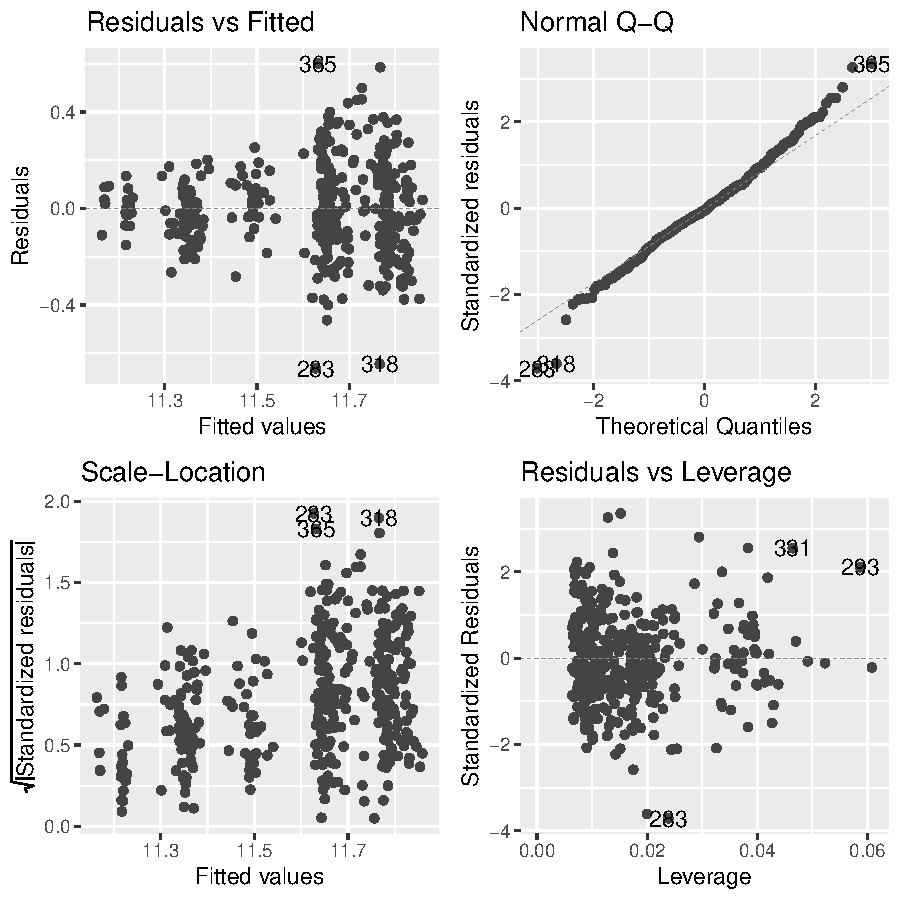
\includegraphics[width=0.6\linewidth]{compulsory_files/figure-latex/fig_model_check_log-transform-1} 

}

\caption{Diagnostic plots for `model2`.}\label{fig:fig_model_check_log-transform}
\end{figure}

\hypertarget{d-interactions-2p}{%
\subsection{d) Interactions (2P)}\label{d-interactions-2p}}

Bert-Ernie hypothesizes that the impact of \texttt{sex} on salary in
academia might be stronger in older generations. While keeping the
log-transformed response and all the other covariates in the model he
therefore decides to design a model with an interaction term between
\texttt{sex} and \texttt{yrs.since.phd}.

\begin{enumerate}
\def\labelenumi{\roman{enumi})}
\tightlist
\item
  Implement the model with the interaction term, and call it
  \texttt{model3} (1P).
\end{enumerate}

\begin{Shaded}
\begin{Highlighting}[]
\NormalTok{model3 }\OtherTok{\textless{}{-}} \FunctionTok{lm}\NormalTok{(log\_salary }\SpecialCharTok{\textasciitilde{}}\NormalTok{ rank }\SpecialCharTok{+}\NormalTok{ discipline }\SpecialCharTok{+}\NormalTok{ yrs.since.phd }\SpecialCharTok{+}\NormalTok{ yrs.service }\SpecialCharTok{+}\NormalTok{ sex }\SpecialCharTok{+}\NormalTok{ sex}\SpecialCharTok{:}\NormalTok{yrs.since.phd }\SpecialCharTok{{-}}\NormalTok{salary, }\AttributeTok{data =}\NormalTok{ Salaries)}
\FunctionTok{summary}\NormalTok{(model3)}
\end{Highlighting}
\end{Shaded}

\begin{verbatim}
## 
## Call:
## lm(formula = log_salary ~ rank + discipline + yrs.since.phd + 
##     yrs.service + sex + sex:yrs.since.phd - salary, data = Salaries)
## 
## Residuals:
##      Min       1Q   Median       3Q      Max 
## -0.66187 -0.10831 -0.00951  0.09846  0.60143 
## 
## Coefficients:
##                         Estimate Std. Error t value Pr(>|t|)    
## (Intercept)           11.1537511  0.0591759 188.485  < 2e-16 ***
## rankAssocProf          0.1528200  0.0335575   4.554 7.05e-06 ***
## rankProf               0.4482679  0.0344343  13.018  < 2e-16 ***
## disciplineB            0.1317818  0.0188133   7.005 1.09e-11 ***
## yrs.since.phd          0.0039500  0.0035253   1.120   0.2632    
## yrs.service           -0.0038902  0.0017059  -2.280   0.0231 *  
## sexMale                0.0574914  0.0614436   0.936   0.3500    
## yrs.since.phd:sexMale -0.0007049  0.0031407  -0.224   0.8225    
## ---
## Signif. codes:  0 '***' 0.001 '**' 0.01 '*' 0.05 '.' 0.1 ' ' 1
## 
## Residual standard error: 0.1809 on 389 degrees of freedom
## Multiple R-squared:  0.5249, Adjusted R-squared:  0.5163 
## F-statistic: 61.39 on 7 and 389 DF,  p-value: < 2.2e-16
\end{verbatim}

\begin{enumerate}
\def\labelenumi{\roman{enumi})}
\setcounter{enumi}{1}
\tightlist
\item
  Interpret the results from \texttt{model3}. Is Bert-Ernie's hypothesis
  correct? (1P)
\end{enumerate}

From the summary of the linear model, we can see that the
\texttt{p}-value for the interaction term is very high, and we conclude
with Bert-Ernie's hypothesis being incorrect.

\hypertarget{e-bootstrap-4p}{%
\subsection{e) Bootstrap (4P)}\label{e-bootstrap-4p}}

You might have noticed that the \(R^2\) we get from \texttt{summary()}
is just a point estimate, without any uncertainty associated to it. We
can use the bootstrap to estimate the uncertainty of the \(R^2\) in our
models. To this end:

\begin{enumerate}
\def\labelenumi{(\roman{enumi})}
\tightlist
\item
  Generate \(1000\) bootstrap samples of the \(R^2\) in \texttt{model1}.
  Use \texttt{set.seed(4268)} at the beginning of the bootstrap
  iterations to ensure that your results are reproducible (2P).
\end{enumerate}

\begin{Shaded}
\begin{Highlighting}[]
\FunctionTok{set.seed}\NormalTok{(}\DecValTok{4268}\NormalTok{)}

\CommentTok{\#Function to extract the R\^{}2{-}value from the linear model}
\NormalTok{getR2 }\OtherTok{\textless{}{-}} \ControlFlowTok{function}\NormalTok{(data, indices) \{}
\NormalTok{  fit }\OtherTok{\textless{}{-}} \FunctionTok{lm}\NormalTok{(salary }\SpecialCharTok{\textasciitilde{}}\NormalTok{ rank }\SpecialCharTok{+}\NormalTok{ discipline }\SpecialCharTok{+}\NormalTok{ yrs.since.phd }\SpecialCharTok{+}\NormalTok{ yrs.service }\SpecialCharTok{+}\NormalTok{ sex, }\AttributeTok{data =}\NormalTok{ data[indices,])}
  \FunctionTok{summary}\NormalTok{(fit)}\SpecialCharTok{$}\NormalTok{r.squared}
\NormalTok{\}}

\FunctionTok{library}\NormalTok{(boot)}
\NormalTok{boot\_results }\OtherTok{\textless{}{-}} \FunctionTok{boot}\NormalTok{(}\AttributeTok{data =}\NormalTok{ Salaries, }\AttributeTok{statistic =}\NormalTok{ getR2, }\AttributeTok{R =} \DecValTok{1000}\NormalTok{, }\AttributeTok{strata =}\NormalTok{ Salaries}\SpecialCharTok{$}\NormalTok{rank)}
\NormalTok{boot\_results}
\end{Highlighting}
\end{Shaded}

\begin{verbatim}
## 
## STRATIFIED BOOTSTRAP
## 
## 
## Call:
## boot(data = Salaries, statistic = getR2, R = 1000, strata = Salaries$rank)
## 
## 
## Bootstrap Statistics :
##      original      bias    std. error
## t1* 0.4546766 0.009072358  0.02803583
\end{verbatim}

\begin{enumerate}
\def\labelenumi{(\roman{enumi})}
\setcounter{enumi}{1}
\tightlist
\item
  Plot the respective distribution of the values (0.5P).
\item
  Find the standard error and the 95\% quantile interval (1P).
\item
  Interpret what you see (0.5P).
\end{enumerate}

Throughout, show your R code and printouts.

\hypertarget{f-picking-a-field-3p}{%
\subsection{f) Picking a field (3P)}\label{f-picking-a-field-3p}}

We (and Bert-Ernie) now assume that \texttt{model1} is the correct (that
is, the data-generating) model. After some character development
(namely, all this R coding is giving him a headache) Bert-Ernie has
figured out that he would rather work in a theoretical field than an
applied field. But, money-conscious as always, he decides that he will
follow this dream if and only if his model predicts that \(20\) years
after finishing his PhD he will be earning \emph{at least} \(75\ 000\)\$
every nine months, with \(95\%\) certainty. He does not care how much he
earns, as long as it is more than \(75\ 000\)\$. He is sure that he will
get a permanent position immediately upon finishing his PhD (so his
\texttt{yrs.since.phd} will equal his \texttt{yrs.service}), that he
will have become full professor within the \(20\) years and that his sex
will still be male.

\begin{Shaded}
\begin{Highlighting}[]
\CommentTok{\# Make a data frame containing two new observations, corresponding to}
\CommentTok{\# Bert{-}Ernie\textquotesingle{}s two possible futures}
\NormalTok{bert\_ernie }\OtherTok{\textless{}{-}} \FunctionTok{data.frame}\NormalTok{(}\AttributeTok{rank =} \FunctionTok{c}\NormalTok{(}\StringTok{"Prof"}\NormalTok{, }\StringTok{"Prof"}\NormalTok{),}
                         \AttributeTok{discipline =} \FunctionTok{c}\NormalTok{(}\StringTok{"A"}\NormalTok{, }\StringTok{"B"}\NormalTok{), }\CommentTok{\# Theoretical, applied}
                         \AttributeTok{yrs.since.phd =} \FunctionTok{c}\NormalTok{(}\DecValTok{20}\NormalTok{, }\DecValTok{20}\NormalTok{),}
                         \AttributeTok{yrs.service =} \FunctionTok{c}\NormalTok{(}\DecValTok{20}\NormalTok{, }\DecValTok{20}\NormalTok{),}
                         \AttributeTok{sex =} \FunctionTok{c}\NormalTok{(}\StringTok{"Male"}\NormalTok{, }\StringTok{"Male"}\NormalTok{))}
\CommentTok{\# Use the full model to predict his salary}
\NormalTok{preds }\OtherTok{\textless{}{-}} \FunctionTok{predict}\NormalTok{(}\AttributeTok{object =}\NormalTok{ model1,}
                 \AttributeTok{newdata =}\NormalTok{ bert\_ernie,}
                 \AttributeTok{interval =} \StringTok{"confidence"}\NormalTok{,}
                 \AttributeTok{level =} \FloatTok{0.975}\NormalTok{) }\CommentTok{\# Not 0.95 since we don\textquotesingle{}t care about upper limit}
\CommentTok{\# Check predictions}
\NormalTok{preds}
\end{Highlighting}
\end{Shaded}

\begin{verbatim}
##        fit      lwr      upr
## 1 116715.6 110985.0 122446.2
## 2 131133.2 126145.6 136120.8
\end{verbatim}

\begin{Shaded}
\begin{Highlighting}[]
\CommentTok{\# Check if lower limit for salary in a theoretical field is large enough}
\NormalTok{preds[}\DecValTok{1}\NormalTok{, }\DecValTok{2}\NormalTok{] }\SpecialCharTok{\textgreater{}} \DecValTok{75000}
\end{Highlighting}
\end{Shaded}

\begin{verbatim}
## [1] TRUE
\end{verbatim}

He sees that the lower limit of the computed interval beats
\(75\ 000\)\$ by a fair amount, so he breathes a sigh of relief.
However, he has made two errors in the call to \texttt{predict()}.

\begin{enumerate}
\def\labelenumi{\roman{enumi})}
\item
  Correct his mistakes, and make the calculation he was actually
  interested in, still using \texttt{predict()}. Will he still be able
  to follow his dream after making the correction, or are many sleepless
  nights of debugging R code looming in his future? (1P)
\item
  Write down an analytic expression for the correct lower limit, and
  implement the analytic expression in R to make sure you get the same
  result as from \texttt{predict()}. (2P)
\end{enumerate}

\textbf{Hint}: see Recommended Exercises Week 3.

\textbf{R-hint}: In the implementation you might have use for the
functions \texttt{model.matrix()}, \texttt{coef()}, \texttt{sigma()},
\texttt{df.residual()}, \texttt{qt()}, \texttt{sqrt()}, \texttt{solve()}
and \texttt{t()}, and the matrix multiplication operator \texttt{\%*\%}.

\hypertarget{problem-3-13p}{%
\section{Problem 3 (13P)}\label{problem-3-13p}}

The Bigfoot Field Researchers Organization (BFRO) is an organization
dedicated to investigating the bigfoot mystery, and for years they have
been collecting reported sightings in a database. They manually classify
their reports into

\begin{itemize}
\tightlist
\item
  Class A: Clear sightings in circumstances where misinterpretation or
  misidentification of other animals can be ruled out with greater
  confidence
\item
  Class B: Incidents where a possible bigfoot was observed at a great
  distance or in poor lighting conditions and incidents in any other
  circumstance that did not afford a clear view of the subject.
\end{itemize}

However, they wonder if this can be automated and done by a
classification algorithm instead. So in this task, you will set up a few
different classification algorithms for this aim, and evaluate their
performance.

Feel free to look at the original data, \texttt{bigfoot\_original}
below, however in this task we will be using a slightly simplified
version of the data set where we have extracted some variables of
interest and deleted observations that are missing any of these
variables of interest.

Download the data as below, and run through the provided
cleaning/preparation steps.

\begin{Shaded}
\begin{Highlighting}[]
\NormalTok{bigfoot\_original }\OtherTok{\textless{}{-}}\NormalTok{ readr}\SpecialCharTok{::}\FunctionTok{read\_csv}\NormalTok{(}\StringTok{"https://raw.githubusercontent.com/rfordatascience/tidytuesday/master/data/2022/2022{-}09{-}13/bigfoot.csv"}\NormalTok{)}
\FunctionTok{library}\NormalTok{(dplyr)}
\CommentTok{\# Prepare the data:}
\NormalTok{bigfoot }\OtherTok{\textless{}{-}}\NormalTok{ bigfoot\_original }\SpecialCharTok{\%\textgreater{}\%}
  \CommentTok{\# Select the relevant covariates:}
\NormalTok{  dplyr}\SpecialCharTok{::}\FunctionTok{select}\NormalTok{(classification, observed, longitude, latitude, visibility) }\SpecialCharTok{\%\textgreater{}\%}
  \CommentTok{\# Remove observations of class C (these are second{-} or third hand accounts):}
\NormalTok{  dplyr}\SpecialCharTok{::}\FunctionTok{filter}\NormalTok{(classification }\SpecialCharTok{!=} \StringTok{"Class C"}\NormalTok{) }\SpecialCharTok{\%\textgreater{}\%}
  \CommentTok{\# Turn into 0/1, 1 = Class A, 0 = Class B:}
\NormalTok{  dplyr}\SpecialCharTok{::}\FunctionTok{mutate}\NormalTok{(}\AttributeTok{class =} \FunctionTok{ifelse}\NormalTok{(classification }\SpecialCharTok{==} \StringTok{"Class A"}\NormalTok{, }\DecValTok{1}\NormalTok{, }\DecValTok{0}\NormalTok{)) }\SpecialCharTok{\%\textgreater{}\%}
  \CommentTok{\# Create new indicator variables for some words from the description:}
\NormalTok{  dplyr}\SpecialCharTok{::}\FunctionTok{mutate}\NormalTok{(}\AttributeTok{fur =} \FunctionTok{grepl}\NormalTok{(}\StringTok{"fur"}\NormalTok{, observed),}
                \AttributeTok{howl =} \FunctionTok{grepl}\NormalTok{(}\StringTok{"howl"}\NormalTok{, observed),}
                \AttributeTok{saw =} \FunctionTok{grepl}\NormalTok{(}\StringTok{"saw"}\NormalTok{, observed),}
                \AttributeTok{heard =} \FunctionTok{grepl}\NormalTok{(}\StringTok{"heard"}\NormalTok{, observed)) }\SpecialCharTok{\%\textgreater{}\%}
  \CommentTok{\# Remove unnecessary variables:}
\NormalTok{  dplyr}\SpecialCharTok{::}\FunctionTok{select}\NormalTok{(}\SpecialCharTok{{-}}\FunctionTok{c}\NormalTok{(}\StringTok{"classification"}\NormalTok{, }\StringTok{"observed"}\NormalTok{)) }\SpecialCharTok{\%\textgreater{}\%}
  \CommentTok{\# Remove any rows that contain missing values:}
\NormalTok{  tidyr}\SpecialCharTok{::}\FunctionTok{drop\_na}\NormalTok{()}
\end{Highlighting}
\end{Shaded}

The data we will use for this task includes the following variables:

\begin{itemize}
\tightlist
\item
  \texttt{class}: the assigned class of the observation, coded as 1 =
  Class A, 0 = Class B
\item
  \texttt{longitude}: longitude of the observation
\item
  \texttt{latitude}: latitude of the observation
\item
  \texttt{visibility}: estimated visibility at the time and place of
  observation (higher value means better visibility)
\item
  \texttt{fur}: does the report contain the word ``fur''?
  \texttt{(TRUE/FALSE)}
\item
  \texttt{howl}: does the report contain the word ``howl''?
  \texttt{(TRUE/FALSE)}
\item
  \texttt{saw}: does the report contain the word ``saw''?
  \texttt{(TRUE/FALSE)}
\item
  \texttt{heard}: does the report contain the word ``heard''?
  \texttt{(TRUE/FALSE)}
\end{itemize}

For the following tasks, we will be using all of these variables.

The data is split into test and training sets as follows:

\emph{Please remember to use the same seed when you split the data into
training and test set.}

\begin{Shaded}
\begin{Highlighting}[]
\FunctionTok{set.seed}\NormalTok{(}\DecValTok{2023}\NormalTok{)}
\CommentTok{\# 70\% of the sample size for training set}
\NormalTok{training\_set\_size }\OtherTok{\textless{}{-}} \FunctionTok{floor}\NormalTok{(}\FloatTok{0.7} \SpecialCharTok{*} \FunctionTok{nrow}\NormalTok{(bigfoot))}
\NormalTok{train\_ind }\OtherTok{\textless{}{-}} \FunctionTok{sample}\NormalTok{(}\FunctionTok{seq\_len}\NormalTok{(}\FunctionTok{nrow}\NormalTok{(bigfoot)), }\AttributeTok{size =}\NormalTok{ training\_set\_size)}
\NormalTok{train }\OtherTok{\textless{}{-}}\NormalTok{ bigfoot[train\_ind, ]}
\NormalTok{test }\OtherTok{\textless{}{-}}\NormalTok{ bigfoot[}\SpecialCharTok{{-}}\NormalTok{train\_ind, ]}
\end{Highlighting}
\end{Shaded}

\hypertarget{a-2p}{%
\subsection{a) (2P)}\label{a-2p}}

\begin{enumerate}
\def\labelenumi{(\roman{enumi})}
\item
  (1P) Fit a \textbf{logistic regression} model using the training set,
  and perform the classification on the test set, using a 0.5 cutoff.
  How many of the reports were classified as clear sightings (class A,
  category 1)?
\item
  (1P) Single choice: According to this model, how would the odds that
  an observation is classified as Class A change if the report contains
  the word ``saw'', compared to if it does not? (all other covariates
  stay the same)
\end{enumerate}

\begin{enumerate}
\def\labelenumi{\arabic{enumi})}
\tightlist
\item
  We multiply by 1.292.
\item
  We multiply it with -3.641.
\item
  We multiply by 0.275.
\item
  We multiply by 3.641.
\item
  We add 3.641.
\item
  We add 1.292.
\end{enumerate}

\hypertarget{b-3p}{%
\subsection{b) (3P)}\label{b-3p}}

\begin{enumerate}
\def\labelenumi{(\roman{enumi})}
\item
  (1P) Fit a \textbf{QDA} model using the training set, and perform the
  classification on the test set, using a 0.5 cutoff. How many of the
  reports were classified as class A?
\item
  (2P) Which statements about linear discriminant analysis and quadratic
  discriminant analysis are true and which are false? Say for
  \emph{each} of them if it is true or false.
\end{enumerate}

\begin{enumerate}
\def\labelenumi{\arabic{enumi})}
\tightlist
\item
  QDA differs from LDA in that it assumes that observations of different
  classes come from Gaussian distributions with different covariance
  matrices.
\item
  LDA is a better choice in cases where there are a lot of observations
  and so reducing bias is important.
\item
  Even if the Bayes decision boundary is linear, QDA will be a better
  choice.
\item
  QDA assumes that the observations are drawn from a multivariate
  Gaussian distribution with common mean vector and class-specific
  covariance matrix
\end{enumerate}

\hypertarget{c-2p}{%
\subsection{c) (2P)}\label{c-2p}}

\begin{enumerate}
\def\labelenumi{(\roman{enumi})}
\tightlist
\item
  (1P) Fit a \textbf{KNN} model using the training set, and perform the
  classification on the test set, with \(k = 25\) (use the \texttt{knn}
  function from the \texttt{class} package).
\end{enumerate}

\textbf{R-hints:} In the \texttt{knn()} function set \texttt{prob=T} to
ensure you get the class probabilities that you then need in d) (change
the ``\texttt{...}'' to the correct input):

\begin{Shaded}
\begin{Highlighting}[]
\NormalTok{knnMod }\OtherTok{\textless{}{-}} \FunctionTok{knn}\NormalTok{(}\AttributeTok{train =}\NormalTok{ ..., }\AttributeTok{test =}\NormalTok{ ..., }\AttributeTok{cl =}\NormalTok{ ..., }\AttributeTok{k =} \DecValTok{25}\NormalTok{, }\AttributeTok{prob =} \ConstantTok{TRUE}\NormalTok{)}
\end{Highlighting}
\end{Shaded}

\begin{enumerate}
\def\labelenumi{(\roman{enumi})}
\setcounter{enumi}{1}
\tightlist
\item
  (1P) Explain how you could choose the tuning parameter \(k\) in a
  better way. How does \(k\) relate to the bias-variance trade-off in
  this context?
\end{enumerate}

\hypertarget{d-6p}{%
\subsection{d) (6P)}\label{d-6p}}

We now wish to compare the performance of the three models (logistic
regression, QDA and KNN) on this dataset, in order to report back to
BFRO on our results.

\begin{enumerate}
\def\labelenumi{\roman{enumi})}
\item
  (2P) In this case, are we interested in prediction or inference? What
  implications would it have for the model choice if we wanted to do
  prediction, and what implications would it have if we wanted to do
  inference? In conclusion, does the question of whether our aim is
  prediction or inference exclude any of the three candidate models in
  this case? (comment briefly)
\item
  (3P) Make confusion matrices for the three predictions performed on
  the test set in a) - c), and report the confusion matrices, along with
  sensitivity and specificity. Explain briefly: What does sensitivity
  and specificity mean? Feel free to explain using the bigfoot example.
  \emph{Make sure it is clear in the confusion matrix which numbers show
  the predictions and which show the true values.}
\item
  (1P) Present a plot of the ROC curves and calculate the area under the
  curve (AUC) for each of the classifiers.
\item
  (1P) Summarize the performance of the three classifiers with words,
  based on the evaluations above. Which one would you choose? Justify
  briefly.
\end{enumerate}

\textbf{R-hints:}

\begin{itemize}
\tightlist
\item
  To obtain \(P(y=1)\) from the \texttt{knn()} output you have to be
  aware that the respective probabilities
  \texttt{attributes(knnMod)\$prob} are the success probability for the
  actual class where the categorization was made. So if you want to get
  a vector for \(P(y=1)\), you have to use \(1-P(y=0)\) for the cases
  where the categorization was 0:
\end{itemize}

\begin{Shaded}
\begin{Highlighting}[]
\NormalTok{probKNN }\OtherTok{\textless{}{-}} \FunctionTok{ifelse}\NormalTok{(knnMod }\SpecialCharTok{==} \DecValTok{0}\NormalTok{,}
                  \DecValTok{1} \SpecialCharTok{{-}} \FunctionTok{attributes}\NormalTok{(knnMod)}\SpecialCharTok{$}\NormalTok{prob,}
                  \FunctionTok{attributes}\NormalTok{(knnMod)}\SpecialCharTok{$}\NormalTok{prob)}
\end{Highlighting}
\end{Shaded}

\begin{itemize}
\tightlist
\item
  You might find the functions \texttt{roc()} and \texttt{ggroc()} from
  the package \texttt{pROC} useful, but there are many ways to plot ROC
  curves.
\end{itemize}

\hypertarget{problem-4-6p}{%
\section{Problem 4 (6P)}\label{problem-4-6p}}

\hypertarget{a-4p}{%
\subsection{a) (4P)}\label{a-4p}}

To calculate the LOOCV statistic when we have \(N\) training data points
we typically have to fit \(N\) models and evaluate the error of each fit
on its left out observation. This task can be computationally intensive
when \(N\) is large. Fortunately, for linear models there is formula for
doing this with fitting just the full data model.

Show that for the linear regression model
\(Y = \mathbf{X} \beta + \varepsilon\) the LOOCV statistic can be
computed by the following formula

\[
\text{CV} = \frac{1}{N} \sum_{i=1}^N \left( \frac{y_i - \hat{y}_i}{1 - h_{i}} \right)^2\ ,
\] where
\(h_i = \mathbf{x}_i^\top \left( \mathbf{X}^\top \mathbf{X} \right)^{-1} \mathbf{x}_i\)
and \(\mathbf{x}_i^\top\) is the \(i\)th row of \(\mathbf{X}\).

\textbf{Hints:}

\begin{enumerate}
\def\labelenumi{\arabic{enumi}.}
\item
  You need to calculate \(\hat{y}_{(-i)},\) which is the predicted value
  of \(y\) when the \(i\)th observation is kept out. This can be written
  as
  \(\hat y_{(-i)} = \mathbf{x}_i^\top \hat{\boldsymbol{\beta}}_{(-i)}\).
\item
  \(\mathbf{X}_{(-i)}^\top \mathbf{X}_{(-i)} = \mathbf{X}^\top \mathbf{X} - \mathbf{x}_i\mathbf{x}_i^\top,\)
  where \(\mathbf{X}_{(-i)}\) is the \(\mathbf{X}\) matrix without the
  \(i\)th row.
\item
  Analogously
  \(\mathbf{X}_{(-i)}^\top \mathbf{y}_{(-i)} = \mathbf{X}^\top \mathbf{y}-\mathbf{x}_i y_i\).
\item
  The
  \href{https://en.wikipedia.org/wiki/Sherman\%E2\%80\%93Morrison_formula}{Sherman--Morrison
  formula} will be useful.
\end{enumerate}

\hypertarget{b-multiple-choice-2p}{%
\subsection{b) Multiple choice (2P)}\label{b-multiple-choice-2p}}

Say for each statement below whether it is true or false.

\begin{enumerate}
\def\labelenumi{(\roman{enumi})}
\tightlist
\item
  The LOOCV will lead to more bias, but less variance than \(10\)-fold
  CV in the estimated prediction error.
\item
  The formula from \textbf{a)} is not valid for polynomial regression.
\item
  The formula from \textbf{a)} is valid when we use the log transform of
  the response in linear regression.
\item
  The validation set-approach is the same as \(2\)-fold CV.
\end{enumerate}

\end{document}
